\documentclass[a4paper,fleqn]{cas-dc}

% If the frontmatter runs over more than one page
% use the longmktitle option.
%\documentclass[a4paper,fleqn,longmktitle]{cas-dc}



\def\tsc#1{\csdef{#1}{\textsc{\lowercase{#1}}\xspace}}
\tsc{SCM}
\tsc{EL}
\tsc{SC}
\tsc{CFB}


%\usepackage[numbers]{natbib}
\usepackage[authoryear]{natbib}
% \usepackage[authoryear,longnamesfirst]{natbib}
\usepackage{booktabs}
\usepackage{caption}
\usepackage{subcaption}
\usepackage[T1]{fontenc}
\usepackage[british]{babel}
\usepackage{microtype}
% \usepackage[tt=false]{libertine}
\usepackage{xcolor}
\usepackage{xurl}
\usepackage{pdfpages}
\usepackage{enumitem}
\usepackage{lineno}
\usepackage{float}
\usepackage{longtable}
\usepackage{geometry}
\usepackage{tabularx}
\usepackage{fontspec}
\setmainfont[Mapping=tex-text,Ligatures={Common,Rare,Discretionary}]{Linux Libertine}

%%%
\begin{document}
\let\WriteBookmarks\relax
\def\floatpagepagefraction{1}
\def\textpagefraction{.001}

% Short title
\shorttitle{T-reX: Quantifying waste and material footprints in LCA}    

% Short author
\shortauthors{McDowall, S2. et~al.}  

% Main title of the paper
\title [mode = title]{T-reX: Quantifying waste and material footprints in current and future Life Cycle Assessment (LCA) databases}  


% First author
%
% Options: Use if required
% eg: \author[1,3]{Author Name}[type=editor,
%       style=chinese,
%       auid=000,
%       bioid=1,
%       prefix=Sir,
%       orcid=0000-0000-0000-0000,
%       facebook=<facebook id>,
%       twitter=<twitter id>,
%       linkedin=<linkedin id>,
%       gplus=<gplus id>]

\author[1]{Stewart Charles McDowall}[orcid=0000-0002-5688-1279]

% Corresponding author indication
\cormark[1]
% Email id of the first author
\ead{s.c.mcdowall@cml.leidenuniv.nl}
% URL of the first author
\ead[url]{scmcd.ch}
% Credit authorship
\credit{Methodology, Software, Validation, Formal analysis, Investigation, Data curation, Writing: original draft, Writing: review \& editing, Visualization}

\affiliation[1]{
  organization={Institute of Environmental Sciences (CML), Leiden University},
  addressline={P.O. Box 9518},
  city={Leiden},
  postcode={2300RA},
  state={South Holland},
  country={The Netherlands}}


\author[1]{Elizabeth Lanphear}[orcid=0009-0003-6364-0873]
\credit{Conceptualization, Methodology, Software, Validation, Writing - review \& editing}


\author[1]{Stefano Cucurachi}[orcid=0000-0003-2748-655X]
\credit{Conceptualization, Writing - review \& editing, Supervision, Project administration, Funding acquisition}


\author[1]{Carlos Felipe Blanco}[orcid=0000-0001-8199-8420]
\credit{Conceptualization, Writing - review \& editing, Supervision, Project administration, Funding acquisition}

% Corresponding author text
\cortext[1]{Corresponding author}


% Here goes the abstract
\begin{abstract}
    The quintessential principle of the circular economy is to minimise material consumption and waste generation. Thus, identifying and quantifying waste and material flows is critical.

    Life Cycle Assessment (LCA) is a powerful quantitative method for this, especially given its capacity to expose the details of an activity's entire life cycle, often guiding the implementation of circular principles to where they could be most effective.
    
    Pursuant to these goals the authors have developed `T-reX', an analytical tool for LCA, written in Python. T-reX extends on the existing computational ecosystem centered on \texttt{Brightway} and \texttt{Premise} and can facilitate the quantification of user-defined supply chain demands for activities in current and prospective scenarios. T-reX streamlines database manipulation for LCA practitioners, integrating methods to aggregate and analyse demand inventories that could expose hotspots of hidden risk.
    
    With a simple case study using lithium-ion batteries, we demonstrate some of T-reX's potential by detailing and exploring aspects of their waste and material footprints. Since such footprints are often linked to negative externalities, T-reX could support sustainable decision-making and contribute to the development of the circular economy by promoting the understanding of our material consumption and waste generation.
\end{abstract}

% Use if graphical abstract is present
\begin{graphicalabstract}
	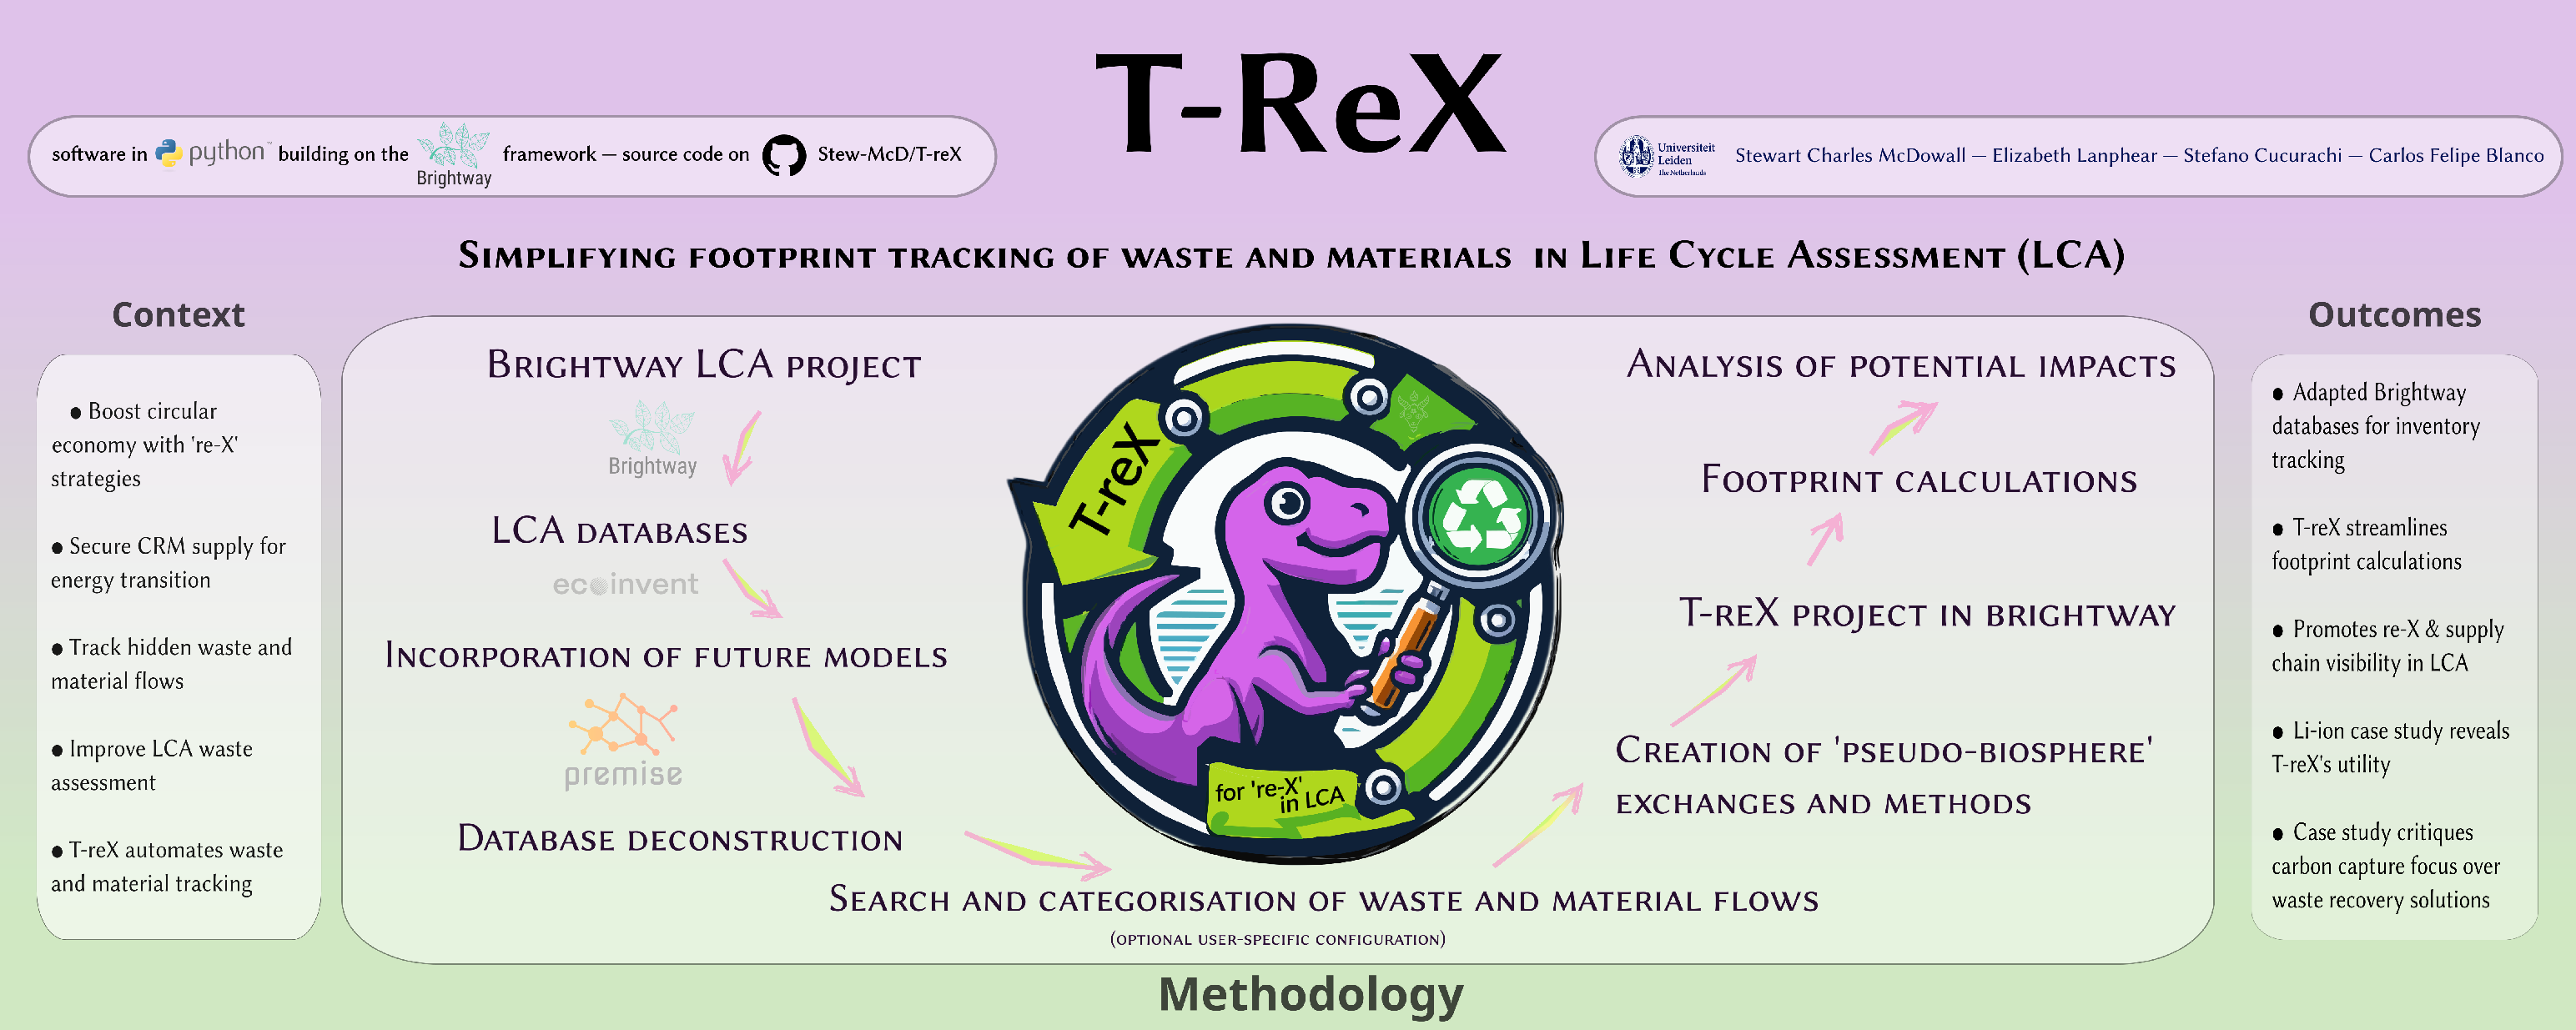
\includegraphics[width=1\columnwidth]{figs/grabs_T-reX_graphical-abstract.pdf}
	%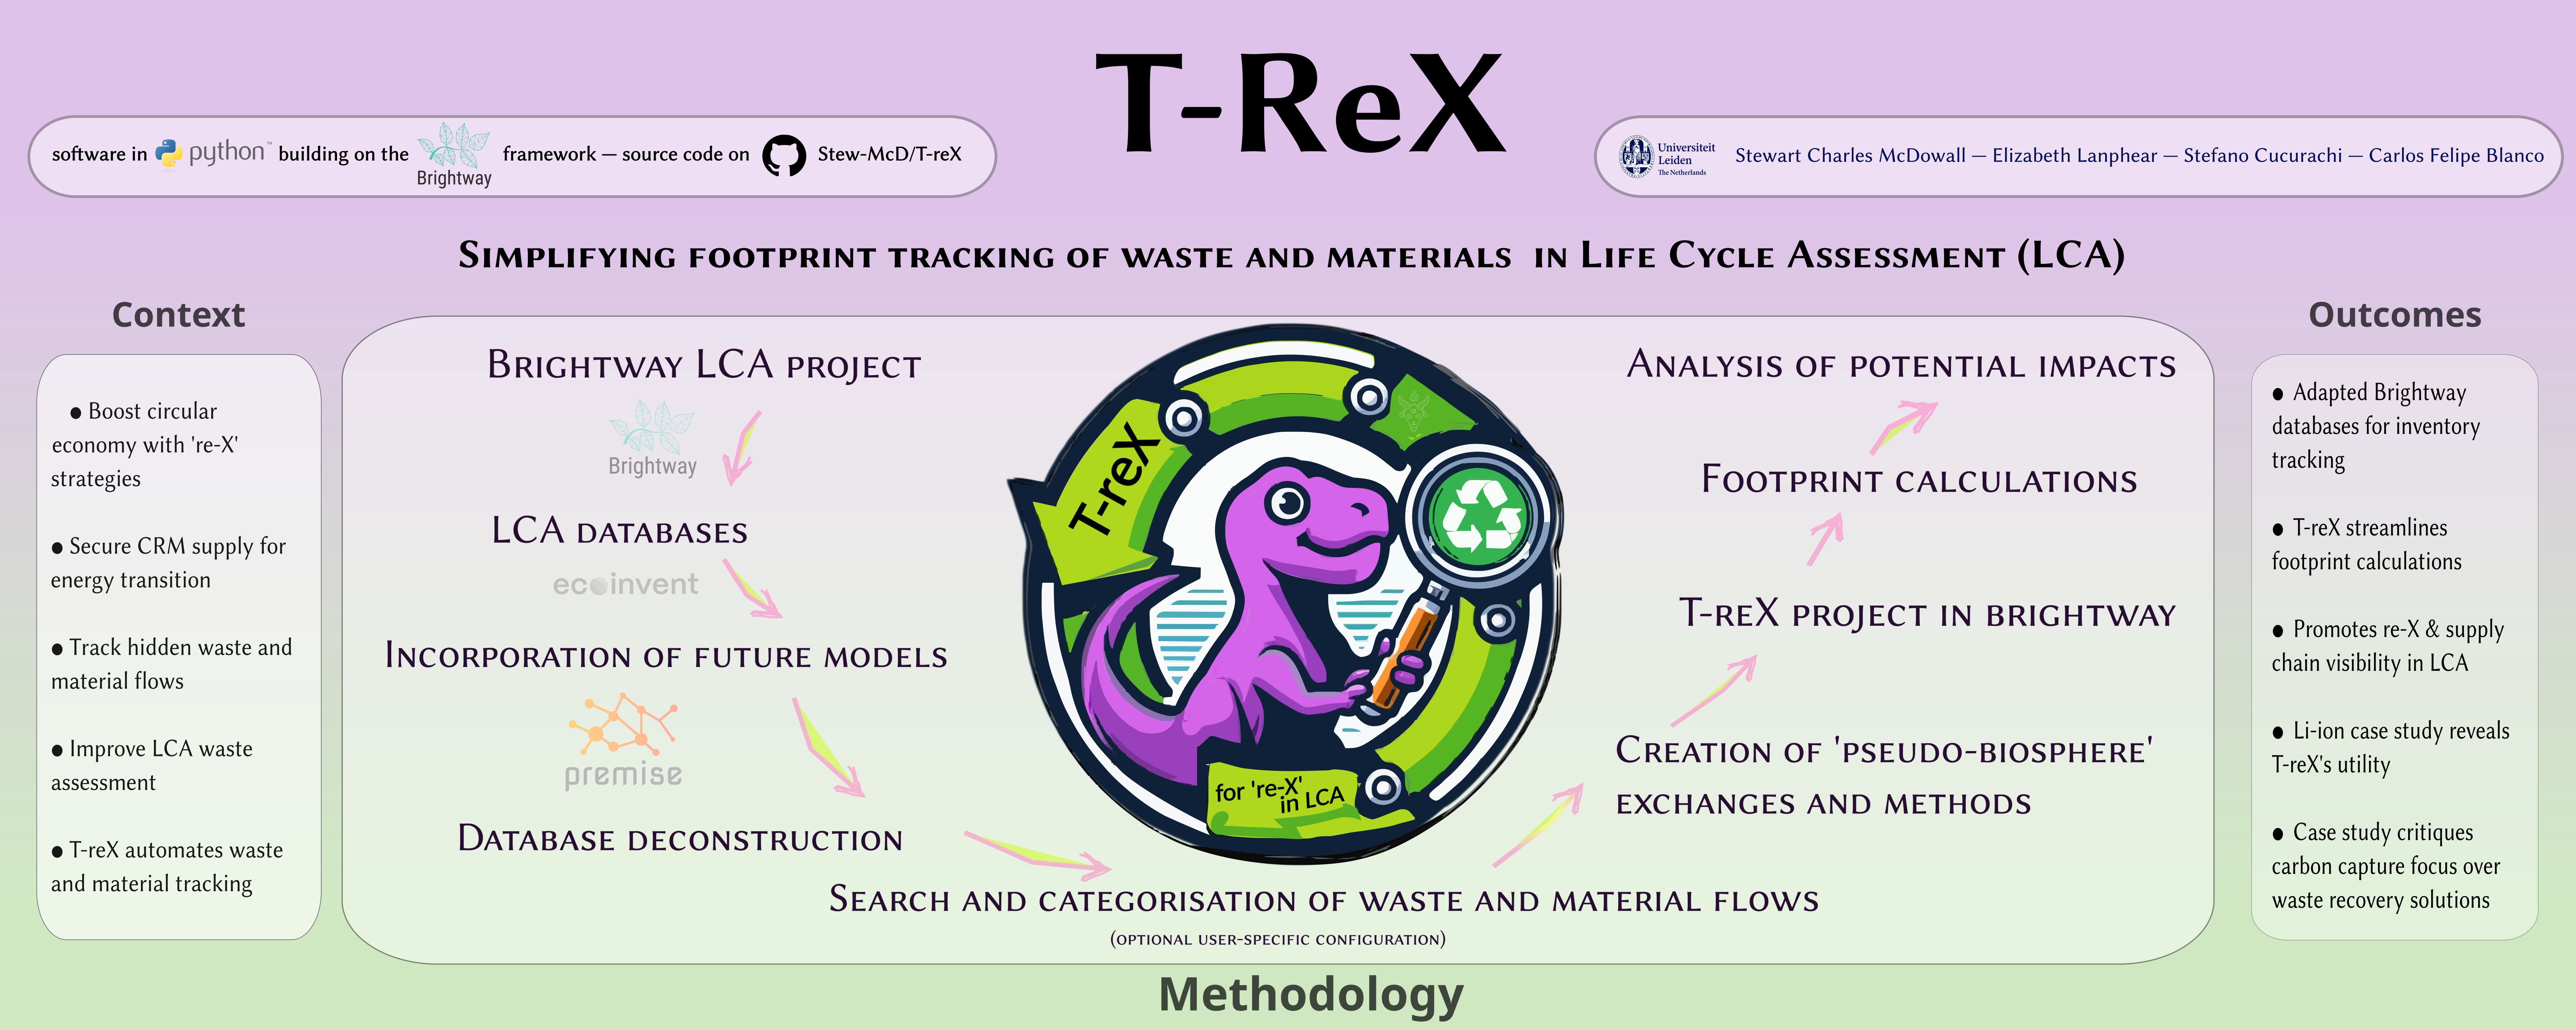
\includegraphics[width=\columnwidth]{figs/grabs_T-reX_graphical-abstract_MID-RES.png}
\end{graphicalabstract}



% Highlights
\begin{highlights}
	\item T-reX, a new open-source program for waste \& material footprints in Life Cycle Assessment (LCA)
	\item Assesses supply risks by calculating demand inventories for critical materials
	\item Simplifies quantification of user-specified waste and material footprint categories
	\item Rapidly identifies hotspots of waste generation and material demand in supply	chains
	\item Presents a case study of five lithium-ion batteries to demonstrate T-reX's potential
\end{highlights}

% Keywords
% Each keyword is seperated by \sep

\begin{keywords}
circular economy\sep waste footprint\sep material footprint\sep life cycle assessment\sep critical raw materials \sep supply chain
\end{keywords}

\maketitle

% Main text
\begin{table*}[!htbp]
	\centering
	\caption{List of abbreviations}\label{tab:abbreviations}
	\begin{tabular}{ll}
		\toprule
		CCS	              & Carbon Capture and Storage                                          \\
		CF                & Carbon Footprint                                                    \\
		EF                & Ecological Footprint                                                \\
		CML               & Centrum voor Milieuwetenschappen (Centre for Environmental Science) \\
		CRM               & Critical Raw Material                                               \\
		CPC               & Cooperative Patent Classification                                   \\
		CSI               & Crustal Scarcity Indicator                                          \\
		CSP               & Crustal Scarcity Potential                                          \\
		EDIP              & Environmental Design of Industrial Products                         \\
		EEIOA             & Environmentally Extended Input-Output Analysis                      \\
		EOL               & End-of-Life                                                         \\
		FOEN              & Swiss Federal Office for the Environment                            \\
		IAM               & Integrated Assessment Model                                         \\
		IE                & Industrial Ecology                                                  \\
		LCA               & Life Cycle Assessment                                               \\
		LCI               & Life Cycle Inventory                                                \\
		LCIA              & Life Cycle Impact Assessment                                        \\
		LFP               & Lithium Iron Phosphate                                              \\
		Li-ion            & Lithium-ion                                                         \\
		LiMn\(_2\)O\(_4\) & Lithium Manganese Oxide                                             \\
		MF                & Material Footprint                                                  \\
		MFA               & Material Flow Analysis                                              \\
		NCA               & Nickel Cobalt Aluminum                                              \\
		NMC               & Nickel Manganese Cobalt                                             \\
		PWF               & Product Waste Footprint                                             \\
		RCP               & Representative Concentration Pathway                                \\
		ReCiPe            & A standard LCIA method set                                          \\
		SDG               & Sustainable Development Goals                                       \\
		SSPs              & Shared Socioeconomic Pathways                                       \\
		T-reX             & The Tool for analysing re-X in LCA                                  \\
		UBP               & Umweltbelastungspünkte (Environmental Impact Points)                \\
		UN                & United Nations                                                      \\
		WF                & Waste Footprint                                                     \\
		\bottomrule
	\end{tabular}
\end{table*}

\section{Introduction}\label{sec:introduction}  
\subsection{Introduction to T-reX}\label{sec:intro-trex}

The development of a circular economy has become a central focus in the pursuit of sustainability objectives toward curtailment of our environmental footprint within planetary boundaries~\citep{eu2019greendeal,eu2020circ,nl2023ceplan,nl2016ceplan,pardo2018ce,ellenmacarthur2015ce}.

Fundamental to this development is a decrease in primary material consumption and a reduction of life cycle waste through the implementation of `re-X'v strategies (e.g., refuse, rethink, design for---and implementation of---repair, remanufacturing and recycling)~\citep{reike2018rex, eu2022ecodesign, eu2022repair, eu2015reman}. In addition to circular economy goals, contemporary geopolitical tensions in an ever more globalised world have highlighted the vulnerability of many advanced economies to intentional supply disruptions---wrought as an act of competition or even outrighthostility~\citep{jrc2023supplychain,hartley2024cepolitics,berry2023crm}.

The concept of the `footprint' as an environmental sustainability indicator began with the Ecological Footprint (EF)~\citep{wackernagel1994ecologicalfootprint} and after being popularised by the Carbon Footprint (CF)~\citep{cucek2015environmentalfootprints} the `footprint family' has adopted many additional metrics---albeit without yet
coalescing into a coherent or consistent framework~\citep{giampietro2014footprintstonowhere,vanham2019footprints,ridoutt2013footprints}. More recently, the footprint
collection has been extended to include the Material Footprint (MF)~\citep{weidmann2013materialfootprint}, which is often encountered in the
`macro methods' of Industrial Ecology (IE), such as environmentally Extended Input-Output Analysis (EEIOA)~\citep{lenzen2022materialfootprint} and Material
Flow Analysis (MFA)~\citep{schaffartzik2013mfafootprint}. Whether at the level of products, entire industries, nations, or even continents, the material
footprint aims to quantify the total material consumed in supply chains. It has been shown that the MF can be `highly representative of damage to human health
and biodiversity'~\citep{steinmann2017resourcefootprints} and indeed, this metric was recently beatified by the United Nations (UN), becoming the `core
official indicator' for targets 8.4 and 12.2 of the Sustainable Development Goals (SDGs)~\citep{lenzen2022materialfootprint}.

Though steadily emerging~\citep{laurenti2016wastefootprint,demirer2019wastefootprint,guillotreau2023wastefootprint}, the `Waste Footprint' (WF) metric is less well-developed. While it seems obvious that reducing life cycle waste is critical to the development of the circular economy~\citep{towa2020wastefootprint,ellenmacarthur2015ce}, the WF remains largely overlooked---especially in LCA models where waste itself is seldom apportioned any inherent environmental significance aside from the emissions related to its treatment~\citep{laurenti2023wastefootprint}. Such neglect strikes the authors as unjustified, given that it has been repeatedly demonstrated that WFs have a strong association with environmental damage~\citep{laurenti2023wastefootprint,doka2024publications, ridoutt2010wasteimpacts,jaio2013wasteabsorbtionfootprint}. Additionally, it has been shown that the most vulnerable communities suffer disproportionately from the social and ecological impacts created by wasteful behaviours and substandard end-of-life treatment~\citep{pellow2023envjusticewaste,akese2018envjustice}.

WF and MF, the two metrics of focus in the study, can provide a comprehensive assessment of potential environmental impacts across the supply chain, encapsulating both resource use and pollution/waste generation, while offering insights at diverse scales, from individual activities to global systems,facilitating communication with a diverse range of stakeholders. Thus, to reduce the negative externalities of human consumption and improve supply chain resilience, it is essential to uncover, disaggregate, and quantify the material and waste footprints of human activities in as much detail as possible~\citep{bisinella2024wastelca,towa2020wastefootprint,berger2020mineralsinlca,sonderegger2020mineralsinlca}.

Life Cycle Assessment (LCA) is a useful method for the holistic estimation of the environmental impacts of products and processes. LCA can comprehensively evaluate impacts across the entire life cycle---from `cradle to grave'--- often identifying critical hotspots and guiding prioritisation of action~\citep{guinee2011lca}. The standard approach is to apply Life Cycle Impact Assessment (LCIA) methods (such as ReCiPe~\citep{huijbregts2016recipe} and CML~\citep{guinee2002cml}), which convert the inventory data into a set of impact scores based on the sum of the elementary flows (those between the technosphere and biosphere). These scores can then be aggregated into one metric for each impact category that can be compared across products and processes. Extending on standard LCA is \textit{ex-ante} LCA, which employs future scenarios to construct `prospective background databases' to predict the impacts of supply chains that have not yet been (and may never be) realised~\citep{cucurachi2018exante,blanco2020exante}.

Several LCIA methods include, to some extent, waste generation (Swiss Eco-Factors, EDIP and EN15804)~\citep{foen2021ecofactors,hauschild2003edip,cen2019en15804} and material consumption (Crustal Scarcity Indicator (CSI) and Swiss Eco-Factors~\citep{arvidsson2020csi,foen2021ecofactors}). These methods, however, are generally limited in their scope (especially for waste), do not allow for flexible quantification of specific waste and material types, and often provide results in characterised units that are abstract or difficult to
interpret (e.g., \textit{Ümweltbelastungspunkte} (UBP) [English: environmental impact points] in the case of the SwissEco-Factors)~\citep{su2020sustainableproddev}.

To facilitate the quantification of waste and material flows in LCA, we
developed a Python package to extend the \texttt{brightway} open-source LCA
framework~\citep{mutel2017brightway} and track these exchanges by translating
them into inventory indicators and `pseudo' LCA impact (LCIA) categories. T-reX
is `T[ool for] re-X' (reduce, reuse, recycle, etc.) and enables LCA
practitioners to manipulate their databases to allow them to easily aggregate
the mass and volume of any desired exchange, and to create flexible categories
that differentiate between material categories, waste types, and treatment or
EOL handling.

Integration with the \texttt{premise} Python
package~\citep{sacchi2022premise}---which connects the projections of
integrated assessment models (IAMs) with current LCA databases---enables the
user to create and manipulate prospective LCA databases. Frustratingly, the
current utility of prospective databases---in general, and in particular for
the waste sector---is constrained by the fact that, to date, the sectoral
coverage of future life cycle inventories (LCIs) is largely confined to energy,
steel, cement, and transport~\citep{sacchi2023premisedocs}. Despite the ever
more critical need to reliably model and future waste management
systems,~\cite{bisinella2024wastelca} reports an alarming lack of coherent
development in this field. \texttt{premise} offers an excellent structure for
the integration of future waste and material flow modelling in LCA databases,
but its potential contribution to the development of the circular economy
cannot be realised if the scientific resources for data collection and
validation are not forthcoming. The authors believe that there is an urgent
need for research investment in this area.


The purpose of T-reX is not to quantify the environmental impacts of material
consumption and waste production (the requisite data and impact modelling
remain lacking), but rather to quantify the material and waste flows
themselves, even those that are finally consumed by waste treatment processes.
It provides, thus, not an impact assessment in the traditional sense, but an
accounting of the material consumed and waste generated by a product or service
inside of the technosphere, regardless of the end-of-life fate of these flows.
By definition, the development of the `circular economy' necessitates the
reduction and ultimate elimination of waste (though whether this objective is
thermodynamically impossible has long been the subject of debate
by~\cite{ayres1998recycling},~\cite{reuter2012recyclinglimits} and many
others). In any case, minimising primary material consumption and the
generation of waste is of paramount importance. By allowing LCA practitioners
to easily classify and quantify these exchanges, T-reX provides a practical
means to identify hotspots and potentially highlight opportunities for waste
reduction and material efficiency.


With the continual improvement of LCA databases and the development of
prospective databases, T-reX can produce ever more realistic estimates,
enhancing its actionable utility derived from the exploration of the potential
impacts of future waste management systems and the material demands of emerging
technologies. The better the data, the more specific and accurate the results
of T-reX analysis, and, thus, the more useful the tool becomes. The authors
hope that T-reX will be a valuable asset to the LCA community and contribute to
the development of a more sustainable and circular economy.

\subsection{Background and need}\label{sec:intro-background}

\subsubsection{Waste in LCA}\label{sec:intro-waste} 

Though often described simply as a `material with a negative economic
value'~\citep{guinee2004economicallocation}, waste is a nebulous concept, and
one whose definition is poorly delineated and highly variable across space and
time. From a systems perspective, the notion of waste is anathema to the
`circular economy', they cannot co-exist. From a practical economic viewpoint,
the viability of an extensive waste processing system is highly dependent on
precise knowledge (or at least, reasonable predictions) of material and waste
flows, in addition to energy costs and the relative prices of virgin and
secondary materials. Thus, as~\cite{bisinella2024wastelca} argues, waste must
be `thoroughly characterised' and `modelling [of its management] must be
physically based'. The reliable, robust models needed to guide the development
of the circular economy can be built only on a foundation of high-quality data.

Accurate and detailed information about waste and waste systems is, by
definition, essential for understanding the `circularity' of a human activity
and for predicting its life cycle externalities. There remains, however, a
knowledge gap regarding WFs and their associated environmental
impacts~\citep{laurenti2023wastefootprint}.

Conventional LCA database models consider waste as a `service' (accounting for
the treatment, not the material)~\citep{guinee2021wasteisnotaservice} and
typically use generic waste processing models~\citep{beylot2018} that break the
causal link between the functional unit and the waste-associated impacts. In
LCA, waste flows are (almost exclusively) not considered as fundamental
biosphere exchanges, but rather, as technosphere flows within the human
economy. Waste produced by an activity is transferred to a relevant waste
treatment activity where it is accepted `burden-free' and transformed into a
combination of emissions and other waste
`products'~\citep{guinee2021wasteisnotaservice}. There can be several treatment
steps in this pathway leading, ultimately, to a mass of material being
deposited in a landfill. In this system of waste accounting, the impacts
apportioned to the waste-producing activity are a sum of those incurred by the
transport, treatment, and final disposal of the waste into terrestrial or
aquatic environments. In particular, the extensive work
of~\cite{doka2024publications} has contributed significantly to understanding
the environmental impacts of waste treatment processes and the modelling of the
long-term impacts of disposal.

A considerable portion of a product's total waste is generated during earlier
stages of its supply chain such as resource extraction, transportation, and
manufacturing, thus, often remaining `invisible' to conventional LCA accounting
practices~\citep{laurenti2016wastefootprint}. This oversight in measuring and
communicating a cradle-to-grave product waste footprint (PWF) highlights a gap
in circular economy indicators. Traditional LCA does not typically view waste
as having environmental significance \textit{per se}, considering instead only
emissions and resource use resulting from waste
treatment~\citep{bisinella2024wastelca, laurenti2023wastefootprint}. The
environmental significance of waste and its correlation with other indicators
has been the subject of extensive research. Studies have shown that popular
resource footprints can cover a significant portion of environmental impact
variance between activities~\citep{steinmann2017resourcefootprints,laurenti2023wastefootprint}.
Correlations between various environmental indicators are not always
consistent, however, as seen with the carbon footprint, which often does not
correlate well with other impact assessment
scores~\citep{laurenti2012carbonfootprint}. The aggregation of waste in PWFs
raises concerns among LCA experts, regarding the uncertainties introduced, as
well as the potential misrepresentation of environmental performance due to
differences in waste
types~\citep{chen2021methoduncertainty,huijbregts2010energyfootprint}.

Some existing LCA methodologies offer direct indicators at the impact
assessment level, but generally, there is little attention given to the impacts
of waste in LCA~\citep{lauran2020abioticdepletion}. This limitation becomes
particularly evident when attempting to identify waste generation hotspots
within a product's life cycle. Addressing these hotspots is crucial for
advancing `circularity', but there is a lack of convenient and flexible methods
to calculate waste flows in LCA and a pressing need for more comprehensive
methods that can effectively quantify waste flows and, therefore, contribute to
a greater understanding of a product's total environmental footprint.

~\cite{laurenti2023wastefootprint} developed a method to calculate the waste footprint of a product or service based on solving the demand vectors of the activities, while also proposing simple measures to quantify waste `hazardousness' and `circularity' with this data. The method presented, as the authors explain, suffers from errors due to double counting due to the way that exchanges are identified and `tagged'. In T-reX, the source database is deconstructed into a list of separate exchanges, and only those explicitly defined as hazardous are marked as such. The `T-reX' Python software tool presented herein provides a more flexible, transparent, and user-friendly approach to quantifying waste flows in LCA\@. Moreover, the utility of T-reX is not limited to waste, it can be used to categorise and aggregate any technosphere exchange of interest (or customised grouping thereof), such as water, gas, and critical raw materials.

\subsubsection{Material demand in LCA}\label{sec:intro-material}

In the context of geopolitical tension and a mineral-hungry `renewable energy
transition', greater attention is being given to the security of material
supply---especially for those considered `critical raw materials'
(CRMs)~\citep{eu2023crmstudy,hool2023crm,mancini2013supplysecurity,jrc2023supplychain,hartley2024cepolitics,salviulo2021supplychain,iea2023crm,iea2023energytechperspectives}.
While LCA seeks to model the technosphere (a.k.a.\ the anthroposphere) and its
exchanges with the biosphere, its focus is often on the environmental impacts
of the system rather than the primary material flows themselves.

The Crustal Scarcity (CSI) LCIA method was developed in order to introduce an
assessment of the long-term global scarcity of minerals in
LCA~\citep{arvidsson2020csi}. The CSI introduced crustal scarcity potentials
(CSPs), which are measured in kg–silicon–equivalents per kg–element and
derived from crustal concentrations. CSPs, provided for 76 elements, reflect
the long-term global elemental scarcity based on crustal concentration proxies.
The CSI, calculated by multiplying CSPs with extracted masses, effectively
gauges the impact of elemental extraction.

While useful for its intended purpose, the CSI presents its results in an
abstract unit (kg-Si eq.) that is difficult to interpret and compare with other
impact categories. Furthermore, the CSPs are not available for all elements (or
more complex materials), and the method does not allow for the quantification
of material demands in terms of mass or volume.


\section{Methodology}\label{sec:methodology}

This section is divided into two parts. In \autoref{sec:method-TreX}, we
describe the T-reX program, and in \autoref{sec:method-casestudy}, we describe
the methodology used to calculate the waste and material inventory footprints
in a case study of five Li-ion batteries, highlighting inconsistencies in LCA
methodology and probing departures from projections in prospective models.

\subsection{T-reX}\label{sec:method-TreX}

\subsubsection{Computational framework}

Developed in the Python programming language, T-reX extends the \texttt{brightway LCA framework}, utilising especially the components
\texttt{bw2data}, \texttt{bw2calc}, and
\texttt{bw2io}~\citep{mutel2017brightway}. Additionally, the \texttt{wurst}
package---which can deconstruct databases into a list of exchanges---is used to
facilitate searching and data transformation at the exchange level (the
individual supply chain flows)~\citep{mutel2017wurst}. Integration with the
\texttt{premise} package~\citep{sacchi2022premise}---which integrates the
projections of integrated assessment models (IAMs) into current LCA
databases---enables the user to easily create and manipulate prospective LCA
databases. T-reX is also compatible with
\texttt{ActivityBrowser}~\citep{steubing2020activitybrowser}---an open-source
graphical user interface for LCA---and after running T-reX, the manipulated
databases and the `pseudo-LCIA' methods created by T-reX can be used in the
project in the accustomed way. T-reX is installable via the Python Package
Index (PyPI)~\citep{mcdowall2023T-reXpipy} and is fully open-source under the
CC-0 licence. The full source code for T-reX is indexed on
Zenodo~\citep{mcdowall2023T-reXzenodo} and under further development in the
GitHub repository~\citep{mcdowall2024T-reXgithub}. T-reX is designed to be used
with \texttt{ecoinvent} databases~\citep{ecoinvent2016version3}, but could be
adapted to other databases by changing the search criteria. Currently, it has
been tested with all available system models of \texttt{ecoinvent}versions
3.5--3.10.

T-reX can be used directly from the command line, or imported as a Python
package with which the user can access the individual functions and modules. In
the simplest case, the user can run the program with the default settings,
which will calculate the waste and material footprint of the
\texttt{ecoinvent}database. The user can adapt the settings of T-reX as
desired, to calculate alternative or additional waste and material inventory
footprints, use a custom database, or a `prospective' database based on future
scenarios by implementing the premise \texttt{premise} with one of T-reX's
internal modules.

The supplementary material in \autoref{sec:supplementary-1} contains metadata of
T-reX, along with a list of the constituent modules, a description of their
functions, and a detailed computational workflow. Further details can be found
in the GitHub repository and in the package documentation~\citep{mcdowall2024T-reXgithub, mcdowall2023T-reXdocs}.

\subsubsection{Functionality and purpose}

T-reX is a Python package that enables one to produce LCA databases---both
current and prospective---that are manipulated to facilitate the calculation of
waste and material inventory footprints in the supply chain of any activity in
the same way as one would apply standard LCIA methods. We refer to the T-reX
methods as `pseudo-LCIA' methods, as they represent an accounting of an
activity's technosphere inventory without reference to impact modelling, as in
standard LCIA.

If desired, prospective databases can be defined by the user or constructed
with the projections of the integrated assessment models such as
IMAGE~\citep{stehfest2014image} and REMIND~\citep{remind2020model}, which offer
a range of options aligned with the Shared Socioeconomic Pathways
(SSPs)~\citep{ssp2020ghg} and can be paired with a variety of mitigation
scenarios.

The deconstruction of the databases by T-reX into lists of exchanges allows the
relevant flows of material and waste to be identified and categorised by the
search functions. The queries facilitating this are tailored to the specific
database and the user can easily modify them to suit their needs. The
categories defined in the configuration are used to create T-reX's `pseudo
LCIA' methods that are indicators of aggregated technosphere demand. The
exchange editing function of T-reX then takes each list of exchanges and
appends to the relevant activity a copy of the technosphere exchange as a
mirrored `pseudo-biosphere' exchange that matches the `pseudo-LCIA' method.

In the default configuration of T-reX, there are 10 waste categories which are
then further divided by their unit of measurement (kilograms and cubic meters)
to create a total of 20 waste methods. The waste categories include
aggregations such as `total waste' `hazardous waste' as well as, those for
`waste sent to treatment' by, for example, incineration or recycling. The full
details are listed in the supplementary material in~\autoref{sec:supplementary-3}. One advantage of T-reX is that it can identify `hidden' waste
exchanges that would otherwise be `consumed' by a treatment process and not
leave the technosphere.

In addition to these waste categories, T-reX can incorporate any number of
material demand categories, the defaults being based on the EU Critical Raw
Materials (CRM) list for 2023~\citep{eu2023crmstudy}, which contains 30
materials considered essential to the EU economy and also at risk of supply
disruption. Especially valuable in the case of CRMs is T-reX's ability to
uncover and quantify these threads of background consumption, which can be
inconspicuously embedded in products or consumed in seemingly distant supply
chain activities. The identity of the materials considered, and their
categorical groupings, are easily customisable by the user. The full list of 59
materials included in the default configuration is provided in the
supplementary material in~\autoref{sec:supplementary-3}.

Following the logic of the standard LCA models~\cite{ecoinvent2016version3, guinee2004economicallocation},
 the identification of material exchanges with
T-reX differs from that used to identify waste exchanges. That is, the search
queries are based on the names of the relevant `market activities' for the
material of interest rather than keywords in the exchange's name. A useful
feature of T-reX is that, in cases where there are several markets for one
material or material grouping, the program can aggregate these flows. For
example, exchanges with markets for the rare-earth-elements (REEs) `market for
cerium', `market for dysprosium', `market for erbium', etc.\ can be aggregated
into a single indicator category for REEs. Similarly, the total demand for all
critical raw materials (CRMs) can be calculated in the same manner.

In these methods, the material demand is calculated based on the total mass
that is extracted from the environment, thus, their focus is essentially solely
on the mining-related exchanges that bring these materials from the biosphere
into the technosphere.

T-reX, in contrast, uses accounting for material demand and waste generation
based on exchanges solely within the technosphere, a material basis. This
offers a different perspective, allowing for the estimation of overall supply
chain material demands that consider the entire life cycle of an activity,
including non-direct effects on the market, such as a `negative consumption' of
other materials due their co-production with the functional unit. Consider a
demand for an activity containing a metal, for example; while the existing
material use methods allow one to calculate the total mass of that metal that
is extracted from the environment, T-reX can provide insight into the broader
supply chain impacts of the demand for this metal. If the production of other
materials is attributed to the production of this metal, these would appear as
negative material demands in the T-reX results---supply chain pressure for one
material can result in lessening of supply chain pressure for another. For
example, in the results of the Li-ion battery case study, this is indeed the
case for nickel demand, which, in the final inventory because of such
co-production, is counter-intuitively negative (due to co-production and
substitution in the LCA system models) despite the presence of nickel in the
final products.

\subsubsection{The workflow of T-reX}

The workflow of T-reX is divided into several modules, each performing a
separate function. The modules are designed to be used in a particular order,
but the user can also use them individually to perform specific tasks. The
standard workflow is as follows:

\begin{enumerate}
	\item Configuration of waste and material exchange categorisation (optional)
	\item Generation of prospective LCA databases (optional)
	\item Database expansion---to create a list of all exchanges in the database
	\item Identification and categorisation of exchanges
	\item Creation of `pseudo-biosphere' databases
	\item Creation of `pseudo-LCIA' methods to calculate waste and material inventory
	      footprints
	\item Exchange editing---whereby the technosphere exchange is mirrored as a
	      `pseudo-biosphere' exchange
	\item Database verification---to ensure that T-reX has manipulated the database
	      correctly
\end{enumerate}

This workflow creates a copy of the original \texttt{brightway} project
containing the original biosphere database, a T-reX `pseudo-biosphere' database
along with one or more manipulated technosphere databases that can be used to
calculate the waste and material inventory footprints of activities in the same
way as standard LCIA calculations.

An overview of the T-reX workflow is presented in
\autoref{fig:methods-flowchart}. The supplementary material in
\autoref{sec:supplementary-3} provides more detailed information.

\begin{figure*}[]
	\centering
	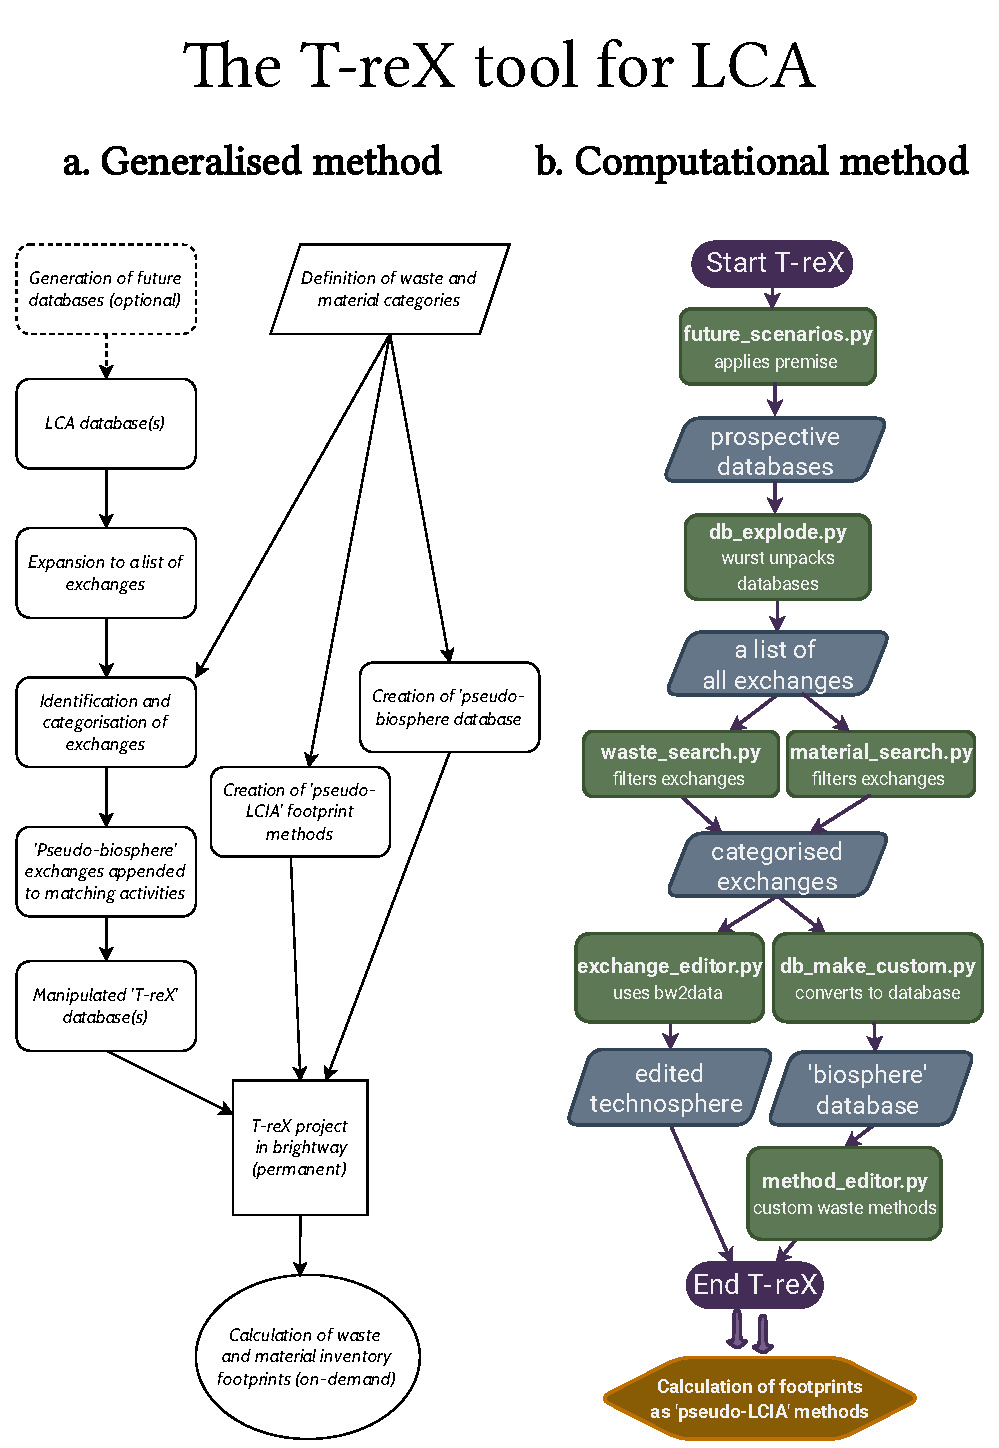
\includegraphics[width=1.8\columnwidth]{figs/T-reX_method.pdf}
	\caption{The workflow of T-reX presented in a generalised (a) and computational (b) format. Application of T-reX to one or more LCA databases creates a \texttt{brightway} project with customised methods and activities that can be used to calculate waste and material inventory footprints of the activity's supply chain.}\label{fig:methods-flowchart}
\end{figure*}

\subsection{Case study methodology}\label{sec:method-casestudy}

To provide an example, we investigated five types of Li-ion batteries in the
\texttt{ecoinvent} 3.9.1 `cutoff' LCA database~\citep{ecoinvent2016version3},
each represented by their unamended global market inventories. The system
boundaries. These following markets were used for the example calculations and
unaltered by the authors:

\begin{itemize}
	\item Li-ion, LFP, rechargeable, prismatic
	\item Li-ion, LiMn\(_2\)O\(_4\), rechargeable, prismatic
	\item Li-ion, NMC111, rechargeable, prismatic
	\item Li-ion, NMC811, rechargeable, prismatic
	\item Li-ion, NCA, rechargeable, prismatic
\end{itemize}

In addition to the waste and material inventory footprint methods created by
T-reX, the following standard LCIA methods were applied for comparison:

\begin{itemize}
	\item ReCiPe 2016 v1.03, midpoint (I)~\citep{huijbregts2016recipe}
	\item Environmental Footprint (EF) v3.1 (no long-term emissions)~\citep{eu2023ef}
	\item Spatial differentiation in life cycle impact assessment---the EDIP 2003 no long term emissions method~\citep{hauschild2003edip}
	\item The crustal scarcity indicator method---CSI 2020~\citep{arvidsson2020csi}
\end{itemize}

Additional to the present-day databases, T-reX created prospective database
sets based on \texttt{ecoinvent} 3.9.1 using the functionality of
\texttt{premise} with the REMIND model and the baseline scenario SSP2 `middle
of the road' with the following Representative Concentration Pathways (RCPs):
\begin{itemize}
	\item SSP2-base: representing an approximate 3.5°C increase in global temperatures to
	      2100
	\item SSP2-PkBudg500: representing the achievement of Paris climate goals, ca. 1.3°C
	      increase to 2100
\end{itemize}

For each pathway, databases (at five-year time intervals) were created with
\texttt{premise}~\citep{sacchi2022premise} and processed with T-reX for the
period between 2020 and 2100.

\subsubsection{LCA calculations}
For each combination of activity, method, and database, a total summation was
calculated along with details of the top contributing processes. Additionally,
for the T-reX methods, a contribution analysis was performed with the
\texttt{bwa.compare\_activities\_by\_grouped\_leaves} function from the
\texttt{brightway2\_analyzer} package~\citep{mutel2016brightway2analyzer}, a
component of the \texttt{brightway} ecosystem. This function performs one
subjective method of graph traversal on the impact matrix of the LCA object to
a specified cutoff. The groups of the resulting `leaves' are collected by their
Cooperative Patent Classification (CPC) codes [giving a representation of
industry sector involvement]. T-reX provides, essentially, a tabulation of
internal exchanges and an insight into the products and sectors in the supply
chain of the activity that carry the most substantial responsibility for the
final waste generation or material demand footprints.



\section{Results}\label{sec:results}
\subsection{T-reX tool}\label{sec:results-T-reX}

An example of the output from the application of T-reX has been included in the
supplementary material~\autoref{sec:supplementary-5}. The
manipulated \texttt{ecoinvent} databases (which are the main product of T-reX)
can be recreated by following the instructions in the package
documentation~\citep{mcdowall2023T-reXdocs}.

\subsection{Case study: Li-ion batteries}\label{sec:results-casestudy}

As described in~\autoref{sec:method-casestudy}, this case study calculated the
waste and material footprints (with a variety of other indicators) for the
unaltered background inventories of five Li-ion batteries with the functional
unit being 1~kg of the battery at the global market. The purpose of this simple
case study was to test, verify, and demonstrate the functionality and
limitations of T-reX. This section includes some highlights of the results,
with full results included in the supplementary material
(\autoref{sec:supplementary-7} and \autoref{sec:supplementary-8}). Because the `pseudo-LCIA' methods created by
T-reX are integrated into the user's \texttt{brightway} project as if they were
standard LCIA methods, the footprint calculations can be performed in the
customary way. In the supplementary material, there are screenshots of selected
results obtained using the \texttt{ActivityBrowser} software, including
contribution analysis and a Sankey diagram that dis-aggregates the final
footprint result over the activities in the supply chain.

\subsubsection{Sankey visualisation of flow inventory footprints}\label{sec:results-case_study-sankey}

\autoref{fig:sankey_waste} presents a heavily abridged Sankey diagram depicting the supply chain flows of `total solid waste' attributed to the NMC 811 Li-ion battery at the global market in the \texttt{ecoinvent} database version 3.9.1. As the supply chains are expansive, this visualisation has been greatly simplified to be legible for print, multiple versions are included in the supplementary material in~\autoref{sec:supplementary-8}. As is evident in the figure, the largest contributors to the waste footprint are the extraction and processing of the raw materials, with the largest flows coming from the extraction of cobalt, lithium, and nickel. Due to the nature of LCA, the waste flows do not represent the `real' physical flows directly, but rather an abstraction thereof based on, in this case, economic allocation---the market price of the functional unit produced by the activity~\citep{guinee2004economicallocation}. If an unallocated database were available, the waste flows could be calculated with T-reX in the same way and would be more directly related to the physical flows of the activities.

\begin{figure}[!htbp]
	\centering
	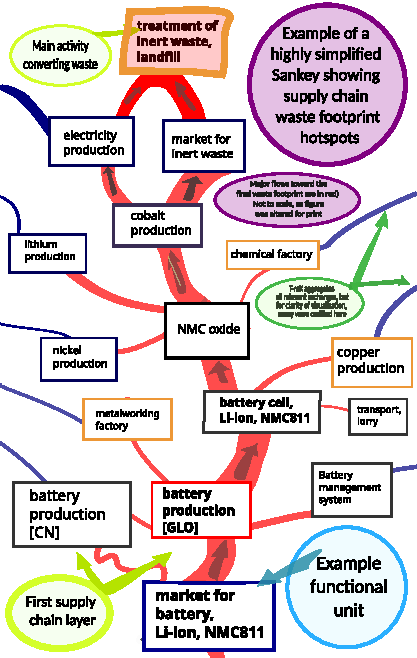
\includegraphics[width=0.8\columnwidth]{figs/T-reX_NMC811_WasteTotalSolid.pdf}
	\caption{A greatly simplified Sankey diagram from \texttt{ActivityBrowser} showing the total solid waste footprint flows for the
	 NMC 811 battery supply chain at the global market in the \texttt{ecoinvent} database version 3.9.1}\label{fig:sankey_waste}
\end{figure} 


\subsubsection{Temporal and scenario variation in waste and material inventory footprints}

%\label{sec:results-case_study-total_footprints}

%! total
\autoref{fig:waste_totalANDcarbon} (a) shows the `total solid waste' inventory footprint for the five Li-ion batteries in the case study from 2020 to 2100 under the SSP2 scenario using the baseline and PkBudg500 RCPs of the REMIND model. The NMC811 battery has the largest footprint, producing over 50~kg of waste per kilogram of battery produced. The  LiMn\(_2\)O\(_4\) battery has the smallest footprint, producing less than 4~kg of waste per kilogram of battery. In each case, there was only a slight downward trend in the waste footprints between 2020 and 2100. This is mostly in the period between 2020 and 2040 and could be attributable to the relatively rapid decrease in fossil fuel use that is factored into the models over this time (since many produce relatively large amounts of waste during extraction and combustion). For the total waste generated by these batteries, there was very little difference observed between the baseline and PkBudg500 RCPs.

%! CO2
The inclusion of carbon capture and storage (CCS) in the prospective databases
is apparent in~\autoref{fig:waste_totalANDcarbon} (b), with the rapid increase
in the production of carbon dioxide `waste' over the period from 2020--2040
that is not seen in the baseline scenario. This result highlights the fact that
the (often) downward trends in global warming impacts calculated with
prospective databases using standard LCIA methods are dependent on the
assumptions made about the introduction of CCS technology. The actual
deployment of these technologies was only around 37~Mt CO\(_2\)/yr as of
2023~\citep{dziejarski2023ccs}, far short of the levels projected in many of
the RCP scenarios~\citep{sacchi2023premisedocs}. The authors consider that the
over-representation of CCS and the under-representation of waste processing
technologies in the prospective databases is one significant limitation to the
validity of prospective LCA databases. Significant work is needed to improve
the representation of these technologies in the databases to ensure that the
results are more realistic and useful for decision-making.
%!!!!

\begin{figure*}[!htbp]
	\centering
	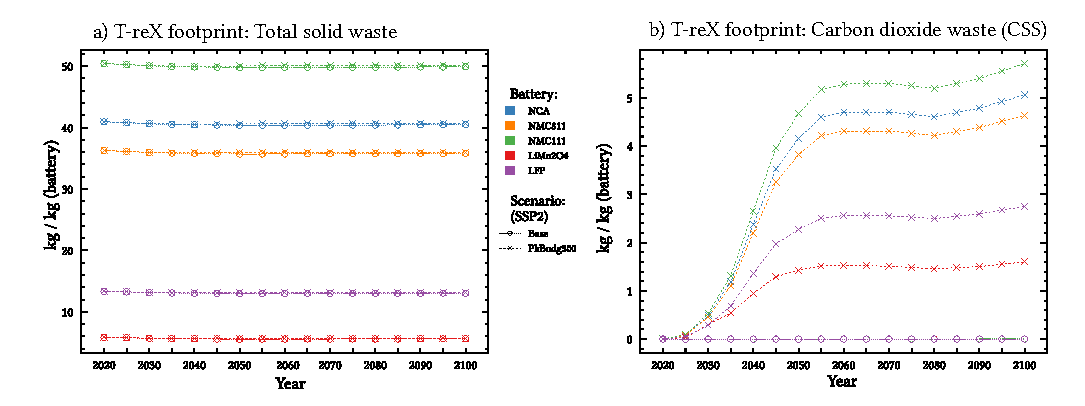
\includegraphics[width=1.8\columnwidth]{figs/T-reX-wastefootprint-totalANDcarbon.pdf}
	\caption{T-reX calculated supply chain inventories for the five Li-ion batteries in the case study, showing their `footprints' for: (a) total solid waste, and (b) carbon dioxide waste (produced from carbon capture and storage (CCS) only). The footprints were modelled with prospective LCA databases from 2020 to 2100 under the SSP2 scenario using the baseline and PkBudg500 RCPs of the REMIND model.}\label{fig:waste_totalANDcarbon}
\end{figure*}


\subsubsection{Contribution of `top-processes' in the supply chain}\label{sec:results-case_study-topprocesses}

\autoref{fig:top_contribution} shows the contribution of the `top-processes' to the graphite footprint of the  LiMn\(_2\)O\(_4\) battery under the baseline scenario from 2020--2100. The total footprint is seen to more than triple, from 0.16~kg/kg in 2020 to 0.52~kg/kg in 2050 and onward to 2100. The largest contributor is not, in this case, the battery-embedded graphite electrode (which is the second top process), but `silicon production' from further up in the supply chain. This result is likely a reflection of the electrification of the transport and energy sectors that is included in the REMIND model. The results of this kind of analysis with T-reX can be used to identify the most significant processes in the supply chain and to target interventions to reduce the potential environmental impact of production.

\begin{figure}[!htbp]
	\centering
	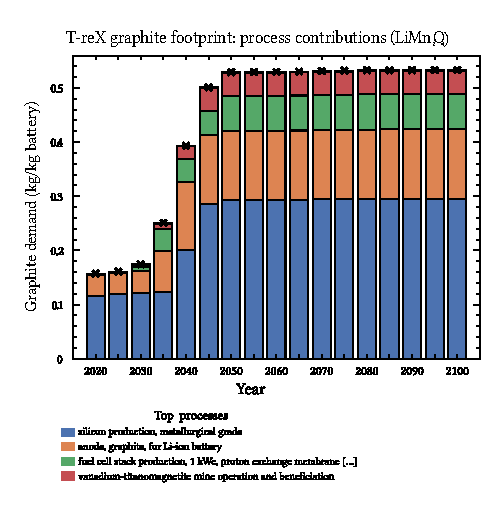
\includegraphics[width=0.8\columnwidth]{figs/T-reX-wastefootprint-processcontributions.pdf}
	\caption{Contribution by the `top-processes' to graphite demand inventory of the LiMn\(_2\)O\(_4\) battery from 2020 to 2100 under the SSP2 scenario using the baseline RCPs of the REMIND model}\label{fig:top_contribution}
\end{figure} 



\subsubsection{Contribution of industrial sectors in the supply chain}\label{sec:results-case_study-topsectors}

\autoref{fig:cpc_contribution} shows the contribution of sectors (grouped by CPC codes) to the total natural gas footprint of the LFP battery under the PkBudg500 pathway. In this example, the relative contribution of the sector `47160: Electronic integrated circuits' is seen to decrease from 11\% in 2020 to 8\% in 2100, while over the same period the contribution of the sector `46430: Parts of primary cells, primary batteries and electrodes' increases from 32\% to 38\%. The method used to calculate these contributions involves traversing the supply chain branches to a certain level (max. 4, in this case), cutting a specified point (5\% in this case), and grouping the value of the `leaves' by their CPC code. The results, therefore, will depend on how deeply the user would like to inspect the supply chain. Additionally, the utility of these results is dependent on how well the CPC codes define the processes in the supply chain for the particular case.

\begin{figure}
	\centering
	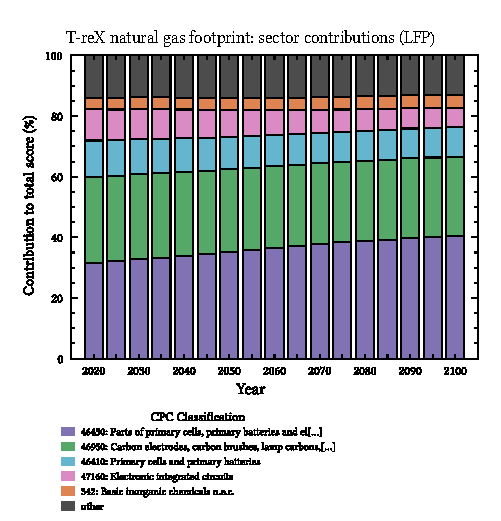
\includegraphics[width=0.8\columnwidth]{figs/T-reX-wastefootprint-sectorcontributions.pdf}
	\caption{Contribution of industrial sectors to the natural gas footprint of the LFP battery from 2020 to 2100 under the SSP2 scenario using the baseline RCP of the REMIND model}\label{fig:cpc_contribution}
\end{figure} 


\subsubsection{Comparison with `similar' LCIA methods}\label{sec:results-case_study-methodcomparison}

A comparison of the results for `Coal (black)' demand using the T-reX method
with the LCIA method `EDIP 2003 – coal no LT' is shown
in~\autoref{fig:comparison_methods}. In this case, both the trends and the
magnitude of the scores were very similar, both demonstrating a general
decrease in the use of coking coal in the battery's footprints. Such
comparability was also observed for other fossil-fuel-related demands (e.g.,
natural gas and petroleum), and to a lesser extent, for some of the metal
demand methods (e.g., zinc and cobalt). Correlation between standard LCIA
methods and T-reX methods is not generally to be expected, however, due to
fundamental differences in the way that the methods are constructed. In
standard LCIA methods, impact scores are derived exclusively from the magnitude
of the exchanges between the biosphere and the technosphere, that is,
extraction and emission. In the T-reX methods, the footprint scores are based
on an accounting of either waste generated or material demand, both of which
are technosphere-technosphere exchanges in terms of LCA modelling. For the
material demand methods especially, this distinction is critical. For example,
the application of the EDIP 2003 or the CSP methods for a given metal will
provide a score that is proportional to the amount extracted by mining, whereas
the T-reX method provides an aggregation of the exchanges with the market for
that metal. The T-reX method, therefore, considers cases of co-production,
recycling, and substitution, providing a picture of the supply chain pressures
that are not captured by the standard LCIA methods. This makes the T-reX
methods more sensitive to the modeling choices (e.g., economic allocation) that
are generally embedded in LCA databases.

\begin{figure*}[!htbp]
	\centering
	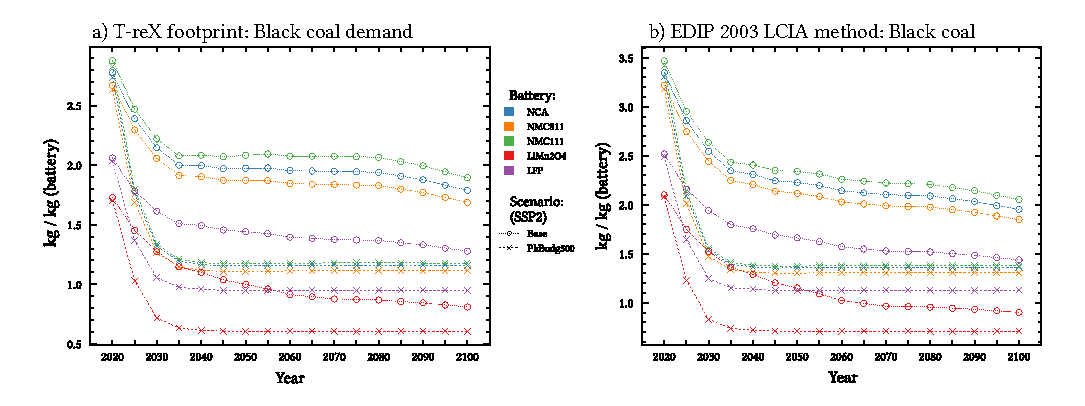
\includegraphics[width=1.8\columnwidth]{figs/T-reX-coalANDedip.pdf}
	\caption{Comparison of the (a) `T-reX – Coal (black)' demand footprint with the (b) conventional LCIA method `EDIP 2003 – coal no longterm'. In the case study from 2020 to 2100 under the SSP2 scenario using the baseline and PkBudg500 RCPs of the REMIND model for all five batteries.}\label{fig:comparison_methods}
\end{figure*}

\subsubsection{Comparison with other studies}\label{sec:results-case_study-comparison}

In the most similar published method,~\cite{laurenti2023wastefootprint} used an
alternative procedure for calculating the waste footprint of \~1400 activities
in the \texttt{ecoinvent} database version 3.5. Direct comparison is not
possible, as this database contains only one generic Li-ion battery, `market
for battery, Li-ion, rechargeable, prismatic'. The inventory of this battery
most closely resembles that of the NMC 111 battery in this case study.
\autoref{tab:results-case_study-comparison} presents a comparison of the
results from the two studies, where possible. For liquid, solid, and recycled
waste, the results were closely aligned, however, for the hazardous waste
fraction, Laurenti et al. reported 95\%, whereas T-reX reported only 3\%. The
reason for this discrepancy is explained by the fact that in the method of
Laurenti et al.\, a ``waste flow was regarded as hazardous when the
hazardousness was clearly stated in its subsequent waste treatment activity''.
The authors continue: ``It should be noted that the high hazardousness ratios
for many products might indicate a weakness in the validity of this measure''.
In T-reX, the source database is deconstructed into a list of separate
exchanges, and only those explicitly defined as hazardous are marked as such.

\begin{table}
	\centering
	\caption{Comparison of the results from the T-reX battery case study (database: \texttt{ecoinvent} 3.9.1 REMIND SSP2 Base 2020, activity: Li-ion NMC 111) with those from \cite{laurenti2023wastefootprint} (database: \texttt{ecoinvent} 3.5, activity:`Li-ion')}\label{tab:results-case_study-comparison}
	\begin{tabular}{lll}
		\toprule
		\textbf{Indicator}         & \textbf{T-reX} & \textbf{Laurenti et al.} \\
		\midrule
		Total solid waste (kg/kg)  & 50.9           & 62.5                     \\
		Total liquid waste (kg/kg) & 3.53           & 3.63                     \\
		Hazardous waste (kg/kg)    & 1.47           & 62.6                     \\
		Recycled waste (kg/kg)     & 1.59           & 1.98                     \\
		\bottomrule
	\end{tabular}
\end{table}

\section{Discussion}\label{sec:discussion}
Waste generation and material demand are strongly associated with the
environmental impacts of human
activities~\citep{laurenti2023wastefootprint,steinmann2017resourcefootprints,
	demirer2019wastefootprint}, and thus must be represented in LCA accounting.
Although there are existing LCIA methods that provide endpoint impact scores
related to material demand and waste generation, they contain convoluted
formulae or subjective weighting, or their complexity and lack of transparency
can make them difficult to use and
interpret~\citep{foen2021ecofactors,hauschild2003edip,cen2019en15804,
	arvidsson2020csi,foen2021ecofactors}.

T-reX advances the state-of-the-art in LCA by providing practitioners with a
simple, flexible, and transparent way to calculate supply chain waste and
material footprints, delivering results in standard units and as direct
aggregations of the relevant demand inventories. Once LCA databases in the
\texttt{brightway} project have been processed with T-reX, the user can easily
apply (and re-apply) the T-reX `pseudo-LCIA' methods to calculate the waste and
material inventory footprints in the same way that they would with a
conventional LCIA method.

The simple case study of five Li-ion batteries presented in this paper
demonstrated the utility, flexibility, and limitations of T-reX.

By adjusting the user configuration for future scenarios and waste/material
categorisation, we produced a set of customised versions of current and
prospective \texttt{ecoinvent} databases along with a `pseudo-biosphere' T-reX
database. Then, by applying the T-reX `pseudo-LCIA' methods, categorised waste
and material inventory footprints for present and future supply chains were
trivial to calculate. Additionally, visual exploration in
\texttt{ActivityBrowser} was possible as the T-reX `pseudo-LCIA' methods are
structurally identical to standard LCIA methods when integrated within the
\texttt{brightway} project.

One limitation of T-reX is that it does not yet provide specific information in
a readily accessible format on the composition of the waste generated. This
information is required to thoroughly assess the potential environmental
impacts of this waste. Currently, the user would need to manually explore the
waste footprint inventory produced by the application of the T-reX to determine
the nature of the waste flows. For example, if the waste generated could
represent an actual loss of resources or potential environmental risk, or, as
is often the case, simply a transfer of the `overburden' in mining activity,
which is classified as `inert waste'. A methodical classification of waste
exchanges and end-of-life fates is expected to be facilitated by the
increasingly detailed and disaggregated data in each successive release of
\texttt{ecoinvent}~\citep{fitzgerald2023ecoinventdocumentation}.

The utility of T-reX in studies of future supply chains is limited by the fact
that the currently available prospective databases focus largely on changes in
the energy, steel, cement, and transport sectors~\citep{sacchi2023premisedocs}.
As demonstrated in the results of the case study---where there were often very
few scenario-temporal changes in many waste and material footprint
indicators---the utility of prospective LCA is restricted if there is
inadequate adoption of future background inventories. In particular, the
inclusion of scenarios with future waste processing technology could greatly
improve our predictions of waste and material flows and offer valuable insight
into their potential impacts~\citep{bisinella2024wastelca}. A strong focus on
enhancing these prospective databases is, thus, of critical importance to the
future of prospective LCA, and by extension, to the development of the circular
economy.

\section{Conclusions}\label{sec:conclusions}

T-reX is an extension to the open-source \texttt{brightway} ecosystem that
enables users to calculate the waste and material footprints of any product or
service in an LCA database. It deconstructs, manipulates and reconstructs the
database to identify and edit waste and material exchanges and writes matching
custom `pseudo' LCIA methods. These exchanges are mirrored in the
\texttt{brightway} project as `pseudo-biosphere' flows and thus, the waste and
material footprints of any other supply chain flow of interest, such as water,
gas, or critical raw materials, can be calculated similarly to existing LCIA
methods.

It is essential that we elucidate the complex relationships between material
demand and waste generation and environmental and social harms. The software we
present in this article enables detailed exploration of `footprints' and life
cycle inventories---modelled externalities of human activities---and examines
their potential connections threats such as supply chain risks and
environmental damage. T-reX is a step towards a better understanding of these
interconnections for the practical realisation of sustainability and the
circular economy.

% Back matter
\appendix
The supplementary material supplied with this manuscript contains the
following sections:
\begin{enumerate}
	\item Metadata of the T-reX Python package\label{sec:supplementary-1}
	\item Details of the modules and user configuration\label{sec:supplementary-2}
	\item Description of the computational workflow\label{sec:supplementary-3}
	\item Modular flowchart of T-reX\label{sec:supplementary-4}
	\item Example of the terminal output of T-reX\label{sec:supplementary-5}
	\item Example of the terminal output of the case study\label{sec:supplementary-6}
	\item Complete tabulated results of the case study\label{sec:supplementary-7}
	\item Complete visualisations from the case study\label{sec:supplementary-8}
\end{enumerate}

\section*{Data availability}
All data used is publicly available online under the noted sources. T-reX is fully open source and dedicated to the public domain under the CC-1.0 licence. It is installable via the Python Package Index (PyPI) under the name `T\_reX\_LCA' \url{https://pypi.org/project/T_reX_LCA}.
The full source code for T-reX is archived by Zenodo at \url{https://zenodo.org/records/10925359} 
and the development server is hosted by GitHub at \url{https://www.github.com/Stew-McD/T-reX}. A user guide with comprehensive documentation are presented at \url{https://T-reX.readthedocs.io}.

\section*{Acknowledgements}
Part of this research project was financially supported by the European Union's Horizon 2020 research and innovation programme under the grant agreement No. 101058522 (project FutuRaM --- futuram.eu). The authors would like to thank the reviewers for their valuable comments and suggestions.

The authors would like to acknowledge those who were part of the futures
thinking small group session at the FutuRaM consortium meeting in Berlin in
June 2023 in which the term `T-reX/T(ool)-reX' was coined to name the vision
presented by Stewart Charles McDowall of a comprehensive open-source software
framework for the study and development of secondary raw material systems. The
authors hope to continue the development of T-reX in the service of our shared
ideals.

\section*{Declaration of competing interest}
The authors declare that they have no known competing financial interests or personal relationships that could have appeared to influence the work reported in this paper.

% To print the credit authorship contribution details
\printcredits

%\section*{CRediT authorship visualisation} % IMPROVED VISUAL VERSION

%\begin{itemize}
%	\item \textbf{SCM}: Stewart Charles McDowall
%	\item \textbf{EL}: Elizabeth Lanphear
%	\item \textbf{SC}: Stefano Cucurachi
%	\item \textbf{CFB}: Carlos Felipe Blanco
%\end{itemize}

\begin{figure}[!htbp]
	\centering
	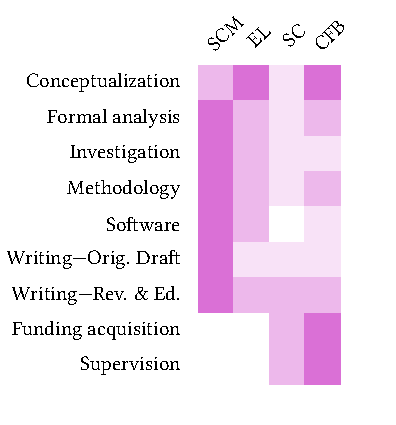
\includegraphics[width=0.8\columnwidth]{figs/T-reX_credit_heatmap.pdf}
	\caption{CRediT authorship visualisation}\label{fig:credit_heatmap}
\end{figure} 


%% Loading bibliography style file
%\bibliographystyle{model1-num-names}
\bibliographystyle{cas-model2-names}

% Loading bibliography database
\bibliography{cas-refs}


\end{document}


